\section{Ethernet und LAN}
\subsection{Local Area Networks (LAN)}

\begin{definition}{LAN}
    Räumlich kleines Netzwerk mit hoher Geschwindigkeit und geringer Latenz
    \begin{itemize}
        \item Auf Schicht 2 (direkte Kommunikation zwischen allen Stationen innerhalb des LAN)
    \end{itemize}
    Vorteile/Möglichkeiten: Gemeinsamer Zugriff (Drucker), Datenaustausch (Directory/File Sharing), direkte Kommunikation (VoIP, Gaming), Zugang zum Internet (über Router im LAN)
\end{definition}

\subsubsection{Topologien}

\begin{definition}{Bus}
    \begin{itemize}
        \item passiv angeschlossene Stationen (konstantes abhorchen, werden aktiv wenn sie senden wollen)
        \item Empfänger erkennt anhand Adresse, ob Daten für ihn sind
    \end{itemize}
\end{definition}

 
    \centering
    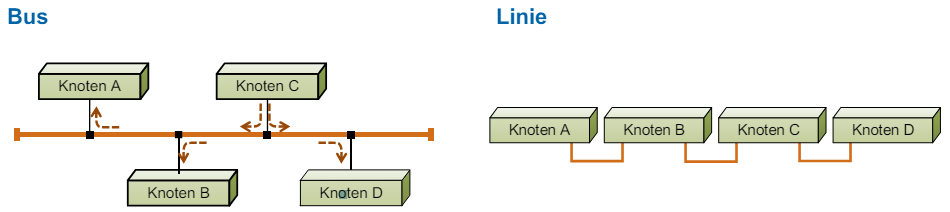
\includegraphics[width=0.9\linewidth]{images/images/bus_linie_topo.png}
 

\begin{definition}{Linien}
    \begin{itemize}
        \item Punkt-zu-Punkt Verbindungen zwischen benachbarten Knoten
        \item Daten empfangen, regenerieren und falls nötig weiterleiten
        \item Ausfall einer Station $\rightarrow$ Segmentierung des LAN in zwei Teile
    \end{itemize}
\end{definition}

\begin{definition}{Ring}
    \begin{itemize}
        \item Achtung: «endloser Kreisverkehr» muss verhindert werden
        \item Gewisse Redundanz: Ausfall einer Station oder Verbindung ok
    \end{itemize}
\end{definition}

 
    \centering
    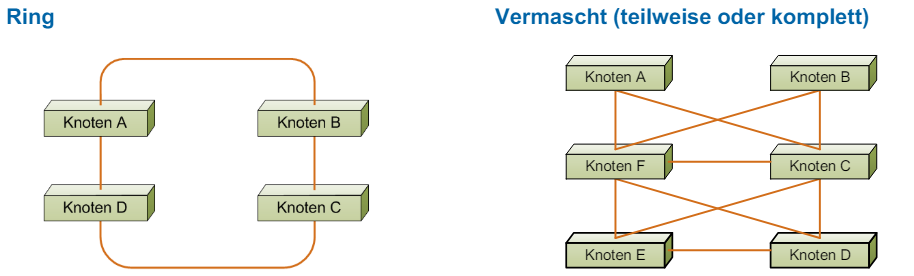
\includegraphics[width=0.9\linewidth]{images/images/ring_vermascht_topo.png}
 

\begin{definition}{Vermascht}
    \begin{itemize}
        \item Hohe Redundanz (Ausfälle können toleriert werden)
        \item hohe Kosten und Aufwand, Achtung: Data duplication
    \end{itemize}
\end{definition}

\begin{definition}{Stern}
\begin{itemize}
    \item Jede Station an zentralen Verteiler angeschlossen
    \item Verteiler entkoppelt Knoten elektrisch und macht LAN weniger störungsanfällig
\end{itemize}
\end{definition}

 
    \centering
    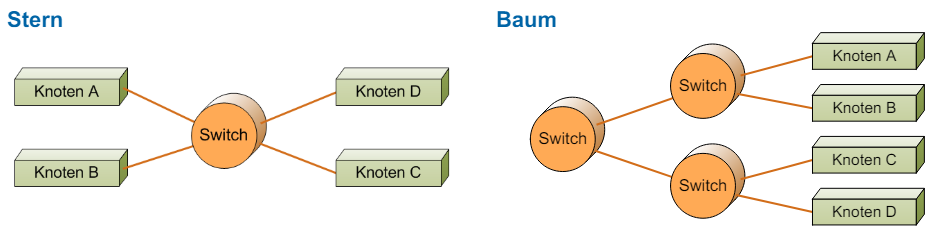
\includegraphics[width=0.9\linewidth]{images/images/stern_baum_topo.png}
 

\begin{definition}{Baum}
    \begin{itemize}
        \item Intelligenten Switches $\rightarrow$ Grossteil der Kommunikation „lokal“
        \item Verringerung der Last für die einzelnen Switches
    \end{itemize}
\end{definition}

\subsubsection{Übertragung und Adressierung}

\begin{definition}{Übertragungsarten}\\
    In jedem Fall: genau 1 Sender
    \begin{itemize}
        \item Unicast: 1 Empfänger, Adresse dieses Empfängers
        \item Multicast: n Empfänger, Multicast-Adresse der Gruppe
        \item Broadcast: alle Knoten im LAN, Broadcast-Adresse des LAN
    \end{itemize}
    \begin{minipage}{0.35\linewidth}
        \includegraphics[width=0.3\linewidth, angle=90]{images/übertragungsarten.png}
    \end{minipage}
    \begin{minipage}{0.6\linewidth}
        Diese Begriffe werden nicht nur im LAN, sondern auch allgemein in Netzwerken verwendet
    \end{minipage}
\end{definition}

\begin{concept}{Adressierung in LANs}
    \begin{itemize}
        \item Jede Station kann Daten von jeder anderen direkt empfangen
        \item Eindeutige Adressen nötig:  erkennen, ob empfangene Daten für die eigene Station bestimmt sind, und wer der Absender ist
        \item IEEE MAC Adressen
        \begin{itemize}
            \item werden nicht konfiguriert
            \item sind fix einem Interface des Gerätes zugeordnet
            \item bestehen aus 6 Bytes
            \item Darstellung hexadezimal 1A-2B-3C-4E-5F-67
        \end{itemize}
        \item Geräte sind möglicherweise mobil und wechseln zwischen LANs, oder LANS werden direkt verbunden $\longrightarrow$ Leitungscode
    \end{itemize}
\end{concept}



\begin{formula}{IEEE MAC Adressen}\\
    Registrierung bei IEEE:
    \begin{itemize}
        \item 3-Byte «OUI» identifiziert Hersteller
        \item 3-Byte Laufnummer durch Hersteller verwaltet
    \end{itemize}
    Die ersten beiden Bits des ersten Adress-Bytes klassifizieren die MAC Adresse\\
    \begin{minipage}{0.6\linewidth}
    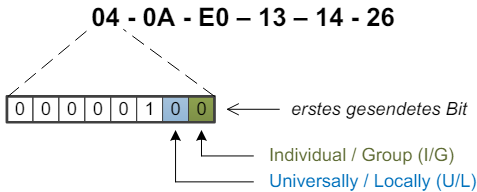
\includegraphics[width=1\linewidth]{images/images/klassifizierung_MAC_adresse.png}
    \end{minipage}
    \begin{minipage}{0.38\linewidth}
    \begin{itemize}
        \item Individual/Group Bit
        \begin{itemize}
            \item 0 = individual address
            \item 1 = group address
        \end{itemize}
        \item Universally/Locally Bit
        \begin{itemize}
            \item 0 = universally administrated adress
            \item 1 = locally administrated adress
        \end{itemize}
    \end{itemize}
    \end{minipage}
\end{formula}

\begin{example2}{Ethernet Frame Format und MAC-Adresse}\\
    Sie senden ein Ethernet Frame über eine 100BASE-TX Schnittstelle und beobachten auf dem Kabel folgende Bit-Sequenz:\\
    10101010 10101010 10101010 10101010 10101010 10101010\\
    10101010 10101011 00010000 00000000 01011010 11100011\\
    10011111 10000110 ...\\
    Wie lautet die MAC-Adresse (in hexadezimaler Darstellung) des Empfängers des Frames und
    wer ist der Hersteller der Ethernet-Karte dieses Empfängers?
    (Hinweis: von den einzelnen Bytes des Frames wird zuerst das LSB und am Schluss das
    MSB übertragen!)
    \begin{itemize}
        \item Zuerst 7 Bytes Präambel (10101010), dann 1 Byte SFD (10101011)
        \item 6 Bytes Destination Address: 00001000 (=08) 00000000 (=00) 01011010 (=5A) 11000111 (=C7) 11111001(=F9) 01100001(=61)
        \item MAC-Adresse: 08-00-5A-C7-F9-61, Hersteller (08-00-5A) IBM
    \end{itemize}
\end{example2}

\subsection*{Ethernet}

\begin{theorem}{Bezeichnungs-Schema}
    Datenraten:\\
    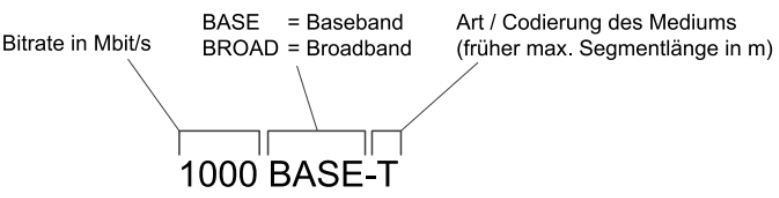
\includegraphics[width=0.8\linewidth]{images/images/ethernet_bezeichnungsschema.png}\\
    \begin{minipage}{0.45\linewidth}
    \begin{itemize}
        \item 10BASE-T: 10 Mbit/s
        \item 100BASE-TX: 100 Mbit/s
        \item 1000BASE-T: 1 Gbit/s
        \item 10GBASE-T: 10 Gbit/s
    \end{itemize}
    \end{minipage}
    \begin{minipage}{0.45\linewidth}
        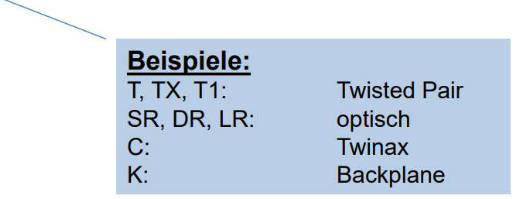
\includegraphics[width=1\linewidth]{images/images/ethernet_bsp_bezeichnung.png}
    \end{minipage}
\end{theorem}

\begin{definition}{Ethernet Frame Format}\\
    Pro Byte wird immer das niederwertigste Bit zuerst und das höchstwertigste Bit zuletzt übertragen. Ausnahme bei Zahlenwerte, z.B. beim Length/Type-Feld.\\
    \begin{minipage}{0.4\linewidth}
        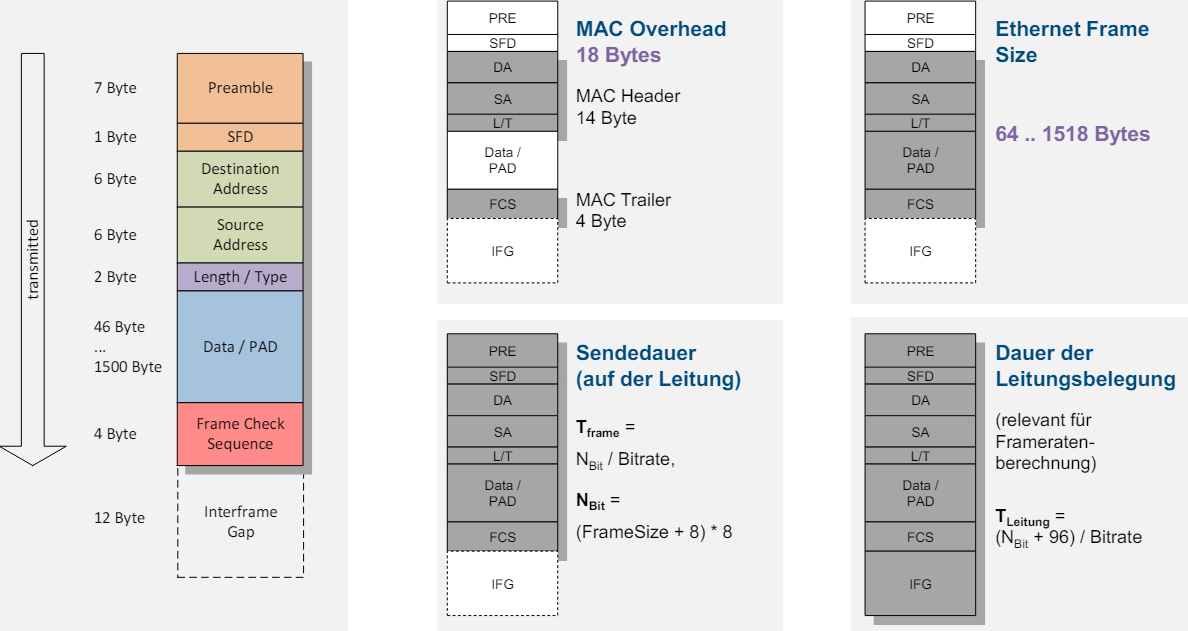
\includegraphics[width=1\linewidth]{images/images/ethernet_format.png}
    \end{minipage}
    \begin{minipage}{0.6\linewidth}
    Length/Type (2 Bytes)
    \begin{itemize}
        \item Fall 1: Länge von DATA ohne PAD ($\leq$ 1500)
        \item Fall 2: Typ von Data = Protokoll der nächsten Schicht ($\leqq$ 1536)
    \end{itemize}
    Data / Padding (46 – 1500 Bytes)
    \begin{itemize}
        \item Enthält die eigentlichen Datenbytes
        \item Bei weniger als 46 Bytes wird mit PAD Bytes abgefüllt
    \end{itemize}
    Frame Check Sequence, FCS (4 Bytes)
    \begin{itemize}
        \item IEEE CRC-32 Algorithmus
    \end{itemize}
    Interframe Gap, IFG (12 Bytes)
    \begin{itemize}
        \item «Zwangspause» zwischen aufeinanderfolgenden Frames
    \end{itemize}
    \end{minipage}
    \vspace{1mm} 
    \begin{center}
        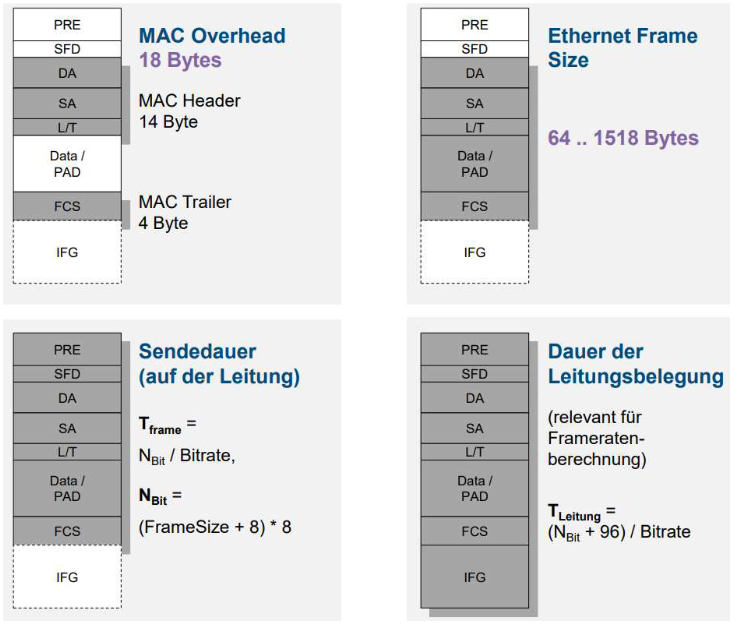
\includegraphics[width=0.8\linewidth]{images/images/ethernet_frame_details.png}
    \end{center}       
\end{definition}

\subsubsection{Ethernet Geräte (Network Gear)}

\begin{definition}{Übersicht Netzwerkgeräte im LAN}\\
    \includegraphics[width=1\linewidth]{images/images/netzwerkgeräte_LAN.png}
\end{definition}


\begin{definition}{Repeater/Hubs im OSI Modell}
    \begin{itemize}
        \item Verstärkt ankommende Signal auf einem Port und leitet sie «in bester Qualität» weiter
        \item VERALTET: Keine Kostenvorteile mehr gegenüber Switches
    \end{itemize}
\end{definition}

\begin{definition}{Switch/Brigde}
    \begin{itemize}
        \item Transparent: sollen für Endgeräte unsichtbar sein
        \item Verwenden «Filtering Database» mit Adress-Learning
        \begin{itemize}
            \item Aufbau und Update der Filtering Database durch Verkehrsbeobachtung (Absenderadresse, nicht Empfänger)
            \item Unbenutzte Einträge werden nach einer gewissen Zeit gelöscht
        \end{itemize}
        \item Port Mirroring möglich
        \item Sicht Endgerät: A und B sind direkt verbunden
        \begin{itemize}
            \item Filtern: nur wenn sicher kein potentieller Empfänger ausgeschlossen ist!!
            \item «Flooding» für Broadcast und Multicast Zieladressen
            \item Unicast: nur an den richtigen Port weiterleiten
        \end{itemize}
    \end{itemize}
\end{definition}

\begin{definition}{Multi-Port-Bridges}
    \begin{itemize}
        \item Daten werden ausschliesslich an den richtigen Port weitergeleitet.
        \item Standard-Komponente zur Kopplung von Segmenten
        \item Werden als Ethernet-Switch bezeichnet
    \end{itemize}
\end{definition}

\begin{definition}{Switch im OSI Modell}\\
    Switch arbeitet auf der Schicht 2: IEEE nennt einen Layer-2 Switch eine Bridge
    \begin{itemize}
        \item Prüft Checksumme und kann Layer-2 Adressen auswerten
    \end{itemize}
    \begin{center}
        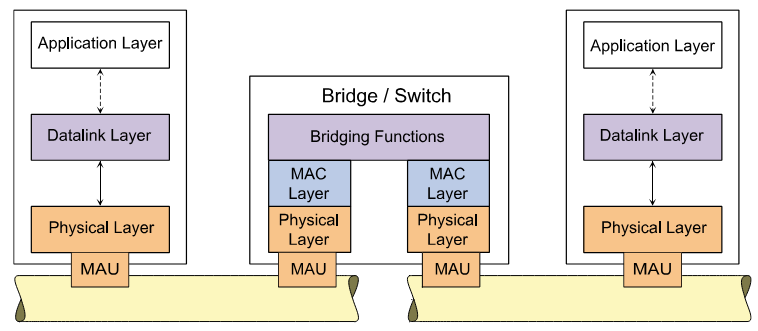
\includegraphics[width=0.8\linewidth]{images/images/switch_osimodell.png}
    \end{center}
\end{definition}

\begin{definition}{Filtering Database}
    Switches verbinden LAN-Segmente\\
    \begin{centering}
        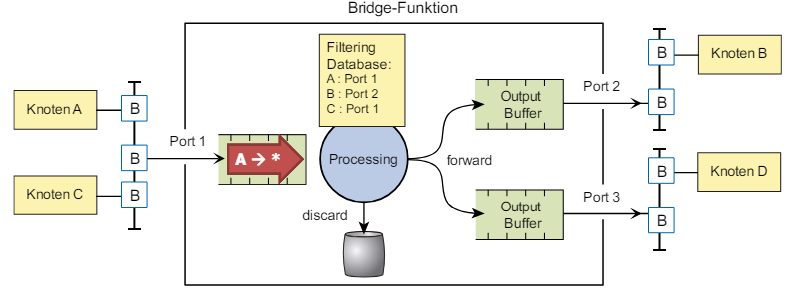
\includegraphics[width=1\linewidth]{images/images/filtering_database.png}    
    \end{centering}
\end{definition}

\begin{KR}{Weg/Zeit-Diagramm für das Senden eines Frames}\\
    Gesamtübertragungszeit (Latenz): $t_{frame} + t_{transfer}$\\
    $t_{forwarding}$ kann verlängert werden um eine Verarbeitungszeit zu ermöglichen\\
        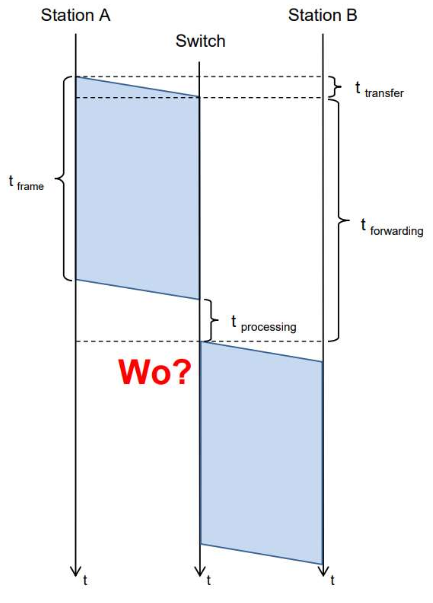
\includegraphics[width=1\linewidth]{images/images/weg_zeit_senden_frame.png}
\end{KR}

\begin{formula}{Senden eines Frames}
    $$t_{frame} = \frac{Framesize}{Bitrate}$$
    $$t_{transfer} = \frac{d_{max}}{C_{Medium}} = \frac{Distanz}{2/3 Lichtgeschw.}$$
\end{formula}

\begin{formula}{Kollisionserkennung}
    können durch Überlagerung von Signalen entstehen. Kollisionen müssen erkannt werden!\\
        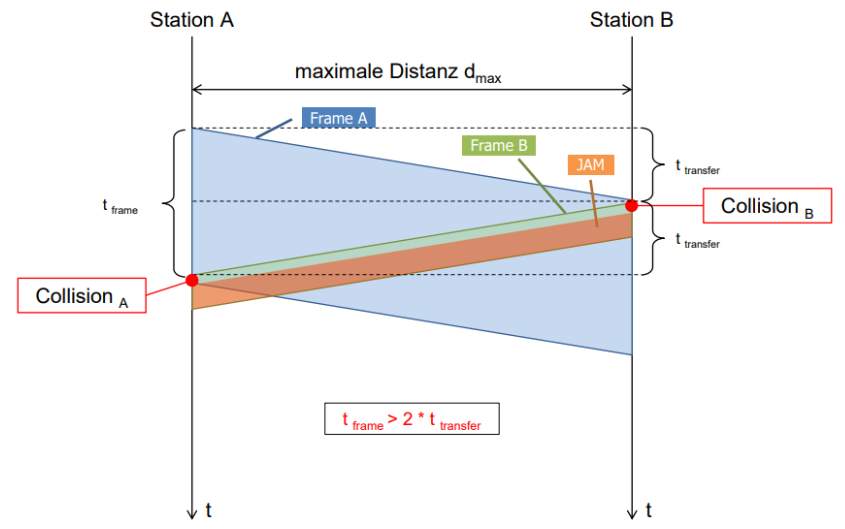
\includegraphics[width=0.9\linewidth]{images/images/kollisionserkennung_lan.png}\\
    Bedingungen für Kollisionserkennung:
    \begin{itemize}
        \item Ohne Repeater: $t_{frame} > 2 \cdot t_{transfer}$
        \item Mit Repeater: $t_{frame} > 2 \cdot (\sum t_{transfer} + \sum t_{forwarding})$
    \end{itemize}
    Ein Knoten kann Kollisionen nur lokal erkennen, solange er selbst am Senden ist
    $$d_{max} < \frac{1}{2} \cdot \frac{Framesize_{min}}{Bitrate} \cdot C_{Medium}, d_{max} < \frac{1}{2} \cdot \frac{576 Bit}{10 \cdot 10^6 \cdot Bit/s}$$
\end{formula}

\columnbreak

\subsubsection*{CSMA/CD}

\begin{concept}{Repeater and Collision Domain}\\
    Eine Collision Domain ist ein Teilbereich eines LANs, in dem die Frames der Stationen miteinander kollidieren können.
    Besteht aus über einen Repeater verbundenen Segmenten.
    \begin{itemize}
        \item Erkennen von Kollisionen
        \begin{itemize}
            \item Halbduplex Collision Detection Unit
            \item Vollduplex Keine Kollisionen
        \end{itemize}
        
        \item Repeater/Hub
        \begin{itemize}
            \item erkennt Kollisionen wenn gleichzeitig von mehreren Ports Frames empfangen werden
            \item Ankommendes Signal wird an alle anderen Ports weitergeleitet, regeneriert und ausgesendet. 
        \end{itemize}
    \end{itemize}
        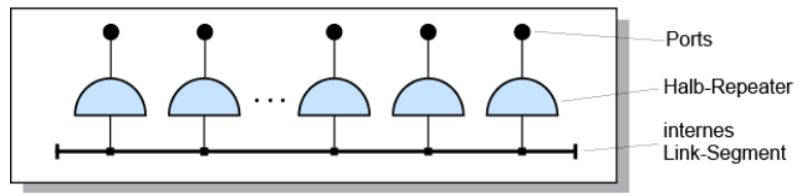
\includegraphics[width=0.75\linewidth]{images/images/repeater_hub.png}
\end{concept}



\begin{KR}{Key Takings LAN/Ethernet Basics}
    \begin{itemize}
        \item Alle Ethernet Varianten
        \begin{itemize}
            \item Definieren die physikalische und Teile der Sicherungsschicht
            \item verwenden das gleiche Frame-Format, das auch in allen später entwickelten Ethernet/802.3 -Varianten verwendet wird
            \item MAC-Adressen der Länge 6 Bytes identifizieren Ethernet Geräte
        \end{itemize}
        \item Switches (Bridges) arbeiten transparent (unsichtbar) auf dem Data Link Layer und schliessen mehrere Segmente zu einem LAN zusammen
        \begin{itemize}
            \item Bridges leiten (Address Learning) Frames nur dorthin weiter, wo sie empfangen werden müssen $\longrightarrow$ Lastreduzierung und Erhöhung der effektiv nutzbaren Kapazität
        \end{itemize}
    \end{itemize}
\end{KR}

\columnbreak

\subsubsection{Redundanz (Spanning Tree)}

\begin{concept}{Redundanz}\\
    Redundante Pfade schaffen Probleme! $\Rightarrow$ Alle Segmente in einer loop-freien Topologie verbinden
    \begin{itemize}
        \item Ziel: 
        \item Idee:
        \begin{itemize}
            \item Root-Bridge auswählen (willkürliche, aber eindeutige Wahl) 
            \item Ausgehend von der Root einen Baum aufbauen
            \item Redundante Pfade sperren
            \item alle Knoten werden genau einmal verbunden
        \end{itemize}
    \end{itemize}
\end{concept}

\begin{KR}{Spanning Tree Algorithmus}
    Initialisierung
    \begin{itemize}
        \item Alle Ports für Nutzdaten blockiert
        \item Annahme: «Ich bin Root»
        \item Austausch BPDUs mit Nachbarn
    \end{itemize}
    Aufbau des Spanning Tree
    \begin{itemize}
        \item Aufdatieren der Info zu Root (kleinste ID) und Pfadkosten zu dieser
        \item Austausch aufdatierter BPDUs bis Konvergenz
    \end{itemize}
    Setzen der Port Roles
    \begin{itemize}
        \item Freigeben for Nutzdaten von
        \begin{itemize}
            \item Root-Ports (Empfang der «besten» BPDU)
            \item Designated-Ports (Gegenstück zu Root-Ports)
        \end{itemize}
        \item Alle anderen Ports bleiben blockiert (Discarding)
    \end{itemize}
        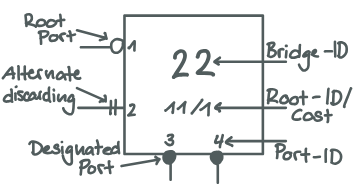
\includegraphics[width=0.75\linewidth]{images/images/spanning_tree_algorithmus.png}\\
        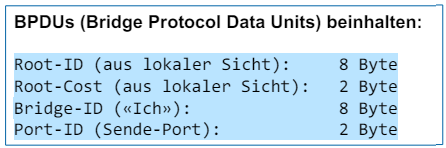
\includegraphics[width=0.5\linewidth]{images/images/bdpus.png}
\end{KR}

\columnbreak

\begin{example2}[breakable]{Rapid Spanning Tree}\\
    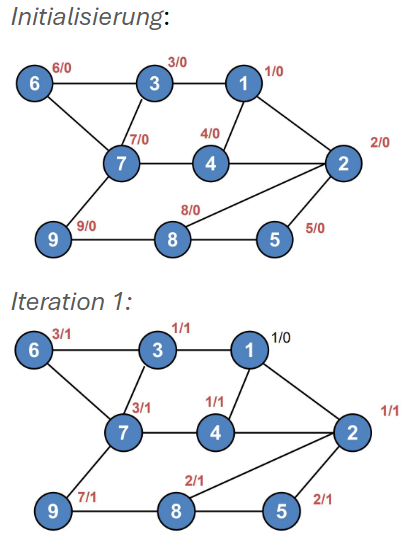
\includegraphics[width=0.7\linewidth]{images/images/rapid_spanning_tree1.png}\\
    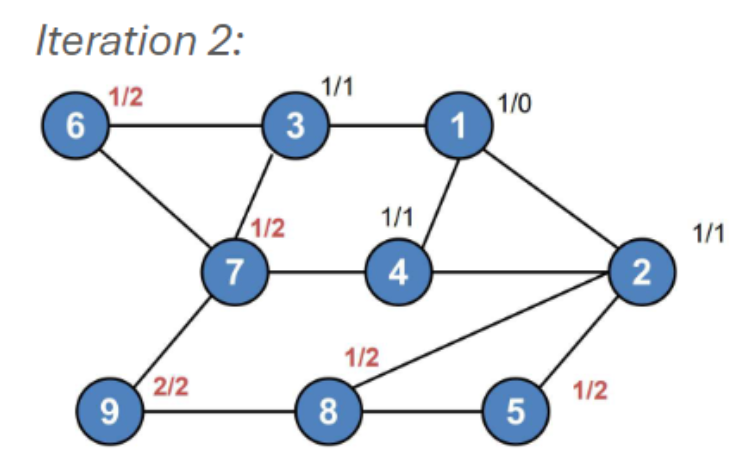
\includegraphics[width=0.7\linewidth]{images/images/rapid_spanning_tree2.png}\\
    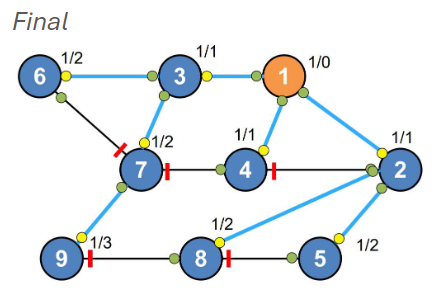
\includegraphics[width=1\linewidth]{images/images/rapid_spanning_tree3.png}
\end{example2}

\columnbreak

\subsection{Virtuelle LANs}

\begin{definition}{VLAN}
    aufteilen eines LANs in mehrere unabhängige logische Netze (Broadcast Domains), unterstützt Prioritäten\\
    Trunk Links: Teil von mehreren VLANs, Frames müssen eindeutig gekennzeichnet werden\\
    \begin{center}
        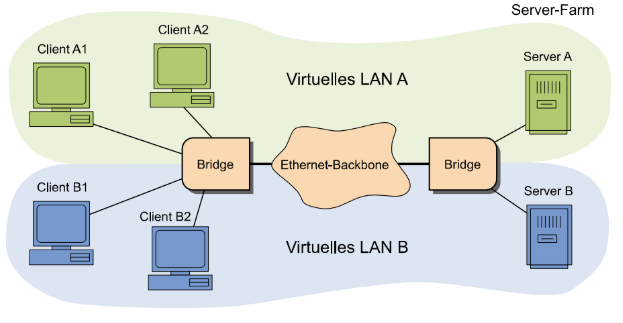
\includegraphics[width=0.8\linewidth]{images/images/vlan.png}\\
    \end{center}
    Trunk = Tagged, Access = Untagged
\end{definition}

\begin{formula}{VLAN Tagging}\\
    Erweiterung des Ethernet Headers durch einen VLAN-Tag
    \begin{itemize}
        \item VLAN-ID (VID) im VLAN-Tag wird zur Zuordnung verwendet
        \item Priority Code Point (PCP) ermöglicht die Priorisierung gewisser Applikationen
        \item Discard Eligibility Indicator (DEI) 0 → Frame wird bei Engpässen zuerst verworfen
        \item VLAN Tagging erfolgt oft beim Eintritt/Austritt ins Netz
        \item Die maximalen Nutzdatenlänge bleibt erhalten, der Ethernet Frame wird 4 Bytes länger
        \item Vorteile:
        \begin{itemize}
            \item Transparent (unsichtbar) für Endgeräte
            \item VLAN Konfiguration nur im Netz
            \begin{itemize}
                \item Einfache zentrale Konfiguration
                \item Einfaches Anpassen der Konfiguration
            \end{itemize}
        \end{itemize}
    \end{itemize}
        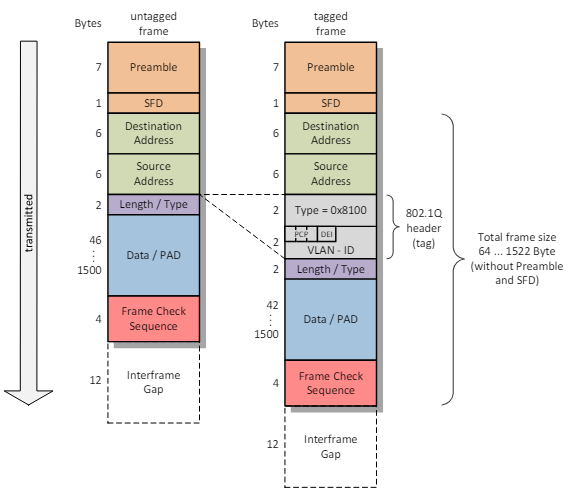
\includegraphics[width=0.8\linewidth]{images/images/vlan_tagging.png}
\end{formula}

\begin{theorem}{Switched LANs: Merkmale von Switches/Bridges}\\
    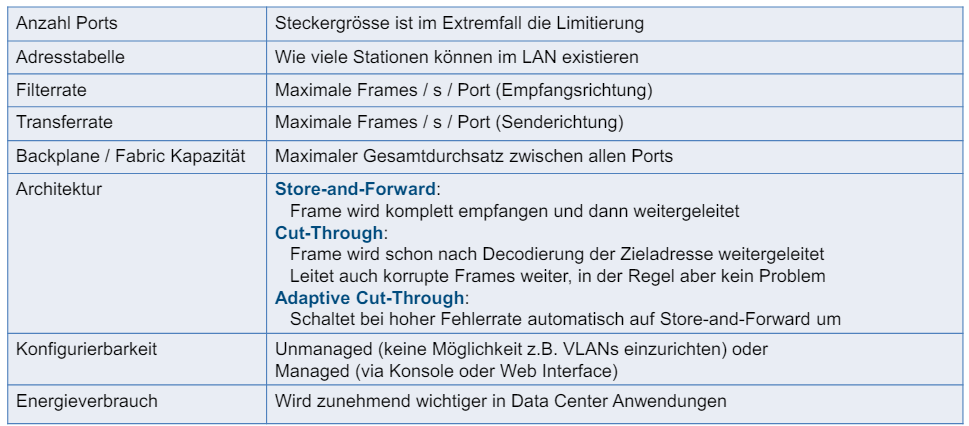
\includegraphics[width=1\linewidth]{images/images/merkmale_switches_bridges.png}
\end{theorem}

\begin{example2}{VLAN Tagging}\\
    Es werden folgende Frames gesendet:
    \begin{center}
        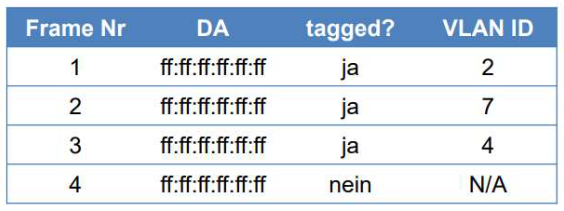
\includegraphics[width=0.6\linewidth]{images/images/bsp_vlan.png}
    \end{center}
    
    Der Switch ist wie folgt konfiguriert:
    \begin{center}
        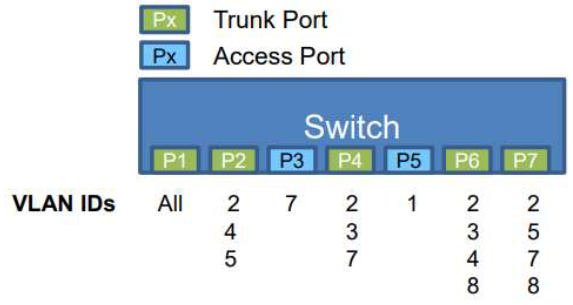
\includegraphics[width=0.6\linewidth]{images/images/vlan_example_switch.png}
    \end{center}
    
    Welche Frames werden an welchen Ports gesendet und sind diese getagged oder ungetagged? Internet Protokolle des Network Layers Das Internet verbindet mehrere LANs miteinander durch Router.
    \begin{center}
        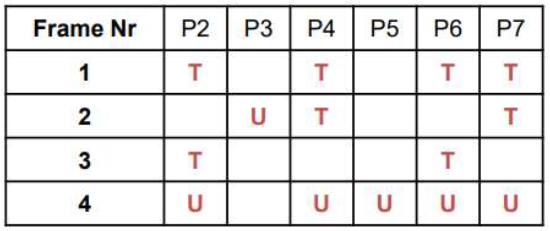
\includegraphics[width=0.5\linewidth]{images/images/vlan_example_frames.png}
    \end{center}
\end{example2}

\begin{KR}{Key Takings Switched LANs}
    \begin{itemize}
        \item Port Mirroring ist ein mögliches Verfahren zur Verkehrsbeobachtung und Fehlersuche in Switched Ethernet
        \item Redundanz wird ermöglicht
        \begin{itemize}
            \item durch die „künstliche“ Reduktion der Topologie au eine aumstruktur durch Spanning Tree Algorithmen
        \end{itemize}
        \item Kompatibilität (10)/100/1000BASE-T wird erreicht durch
        \begin{itemize}
            \item Beibehaltung von Frame Format und Schnittstelle zwischen PHY und MAC
            \item Autonegotiation mittels FLP bursts / NLP
        \end{itemize}
        \item PHY Codierung ist unterschiedlich (Scrambled NRZ/MLT-3 mit 4 5 Codierung, …)
        \begin{itemize}
            \item Höhere Datenrate → höhere Ansprüche an die Signalverarbeitung und Algorithmen im PHY
        \end{itemize}
    \end{itemize}
\end{KR}


\subsubsection*{Switched LANs}


\begin{concept}{Switched LAN Monitoring}\\
    Hub/Multiport Reader
    \begin{itemize}
        \item Pro
        \begin{itemize}
            \item Alle Daten sind auf allen Ports sichtbar
        \end{itemize}
        \item Con
        \begin{itemize}
            \item Verfälscht die Situation völlig
            \item Nur Half Duplex Betrieb für A und B möglich
        \end{itemize}
    \end{itemize}
    Tap/Probe
    \begin{itemize}
        \item Pro
        \begin{itemize}
            \item Sehr detaillierte low-level Analyse möglich
        \end{itemize}
        \item Con
        \begin{itemize}
            \item Kosten
            \item Veränderung des Netzwerkes (Latenz)
        \end{itemize}
    \end{itemize}
\end{concept}

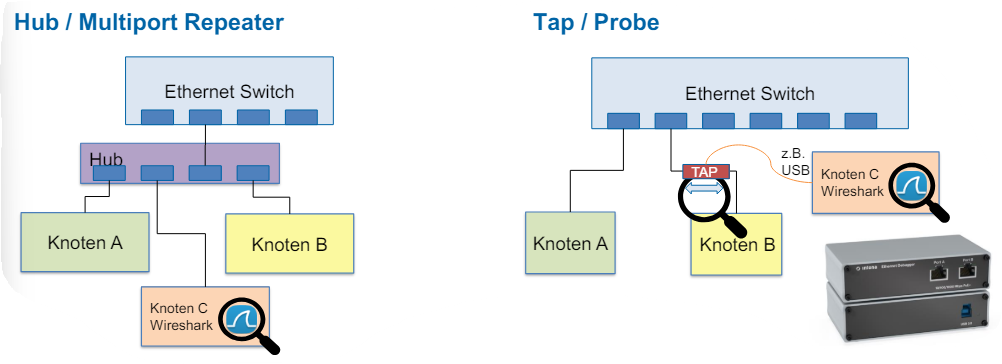
\includegraphics[width=1\linewidth]{images/images/switched_lan_monitoring.png}

\begin{concept}{Port Mirroring}
    Managed Switches unterstützen eine Vielzahl Diagnosefunktionen
    \begin{itemize}
        \item Statistik Zähler pro Port: Anzahl Rx und Tx Frames, FCS-Fehler, zu lange Frames, ...
    \end{itemize}
    Port-Mirroring leitet Daten zusätzlich auf einen anderen Port um
    \begin{itemize}
        \item Konfigurationsoptionen herstellerabhängig
        \begin{itemize}
            \item Kompletter Port (Rx plus Tx), oder selektiv Port Nummer(n) und Richtung
        \end{itemize}
    \end{itemize}
        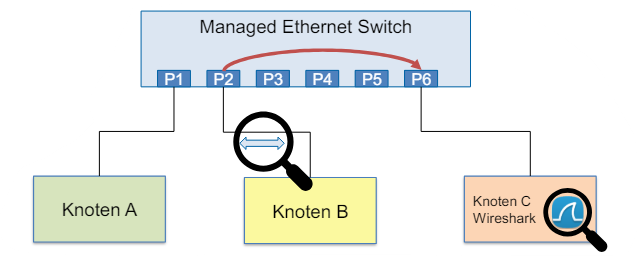
\includegraphics[width=0.6\linewidth]{images/images/port_mirroring.png}
\end{concept}

\begin{concept}{Autonegation}
    Ermittlung der besten Betriebsart durch Austausch der Leistungsmerkmale zweier Netzwerkkomponenten, beruht auf Fast Link Pulses (FLP)
    \begin{itemize}
        \item NLP = Link Presence Detection
        \item FLP = Autonegotiation, Autopolarity
    \end{itemize}
        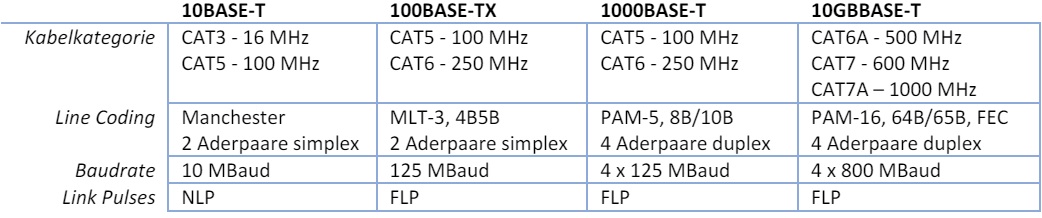
\includegraphics[width=1\linewidth]{images/images/ethernet_systeme.png}
\end{concept}

\begin{formula}{GBASE-T}\\
    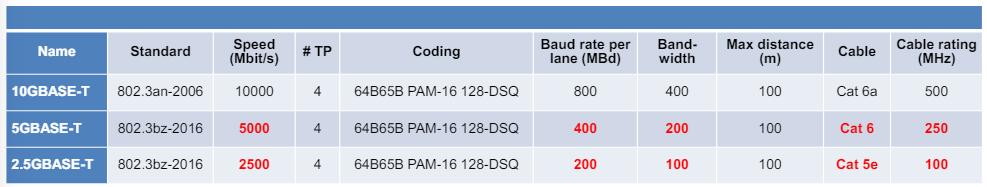
\includegraphics[width=1\linewidth]{images/images/GBASE-T.png}
\end{formula}



